\documentclass[reqno]{amsart}
\usepackage{fancyhdr}
\usepackage{amsmath}
\usepackage{amssymb}
\usepackage{pifont}
\usepackage{booktabs}
\usepackage{subcaption}
\usepackage{graphicx}
\usepackage{verbatim}
\usepackage{hyperref}


\pagestyle{fancy}
\chead{1/7/22}
\rhead{Jackson Dougherty}
\renewcommand{\headrulewidth}{0.4pt}
\renewcommand{\footrulewidth}{0.4pt}

\hypersetup{
    colorlinks=true,     
    urlcolor=blue,
    }

\begin{document}
\section*{Riddler 1-7-22}
\section*{Jackson Dougherty}

\section*{Riddler Classic}

\subsection*{Problem}

Amare the ant is traveling within triangle $\triangle\rm ABC$, shown in fig $\ref{fig:triangleABC}$. Angle $\angle\rm A$ measures $15$ degrees, and sides AB and AC both have length 1. 

\begin{figure}[h]
	\centering
	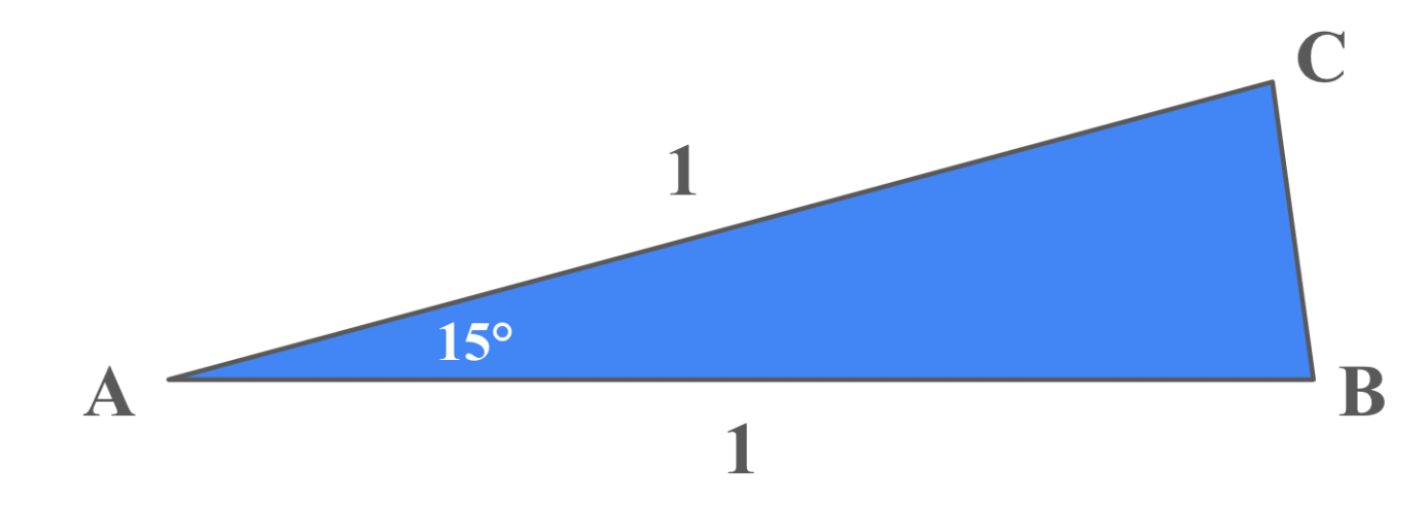
\includegraphics[scale = 0.75]{TriangleABC.png}
	\caption{Amare the ant will travel across triangle $\triangle\rm ABC$.}
	\label{fig:triangleABC}
\end{figure}

Amare starts at point B and wants to arrive on side AC, but the colony's queen requires that Amare's path follow several constraints:
\begin{enumerate}
	\item Start at point B. 
	\item Touch any point on side AC.
	\item Touch any point on side AB.
	\item Reach any point on side AC.
\end{enumerate}

What is the shortest distance Amare can travel while following the queen's path?

\subsection*{Solution}

\begin{figure}[h]
	\centering
	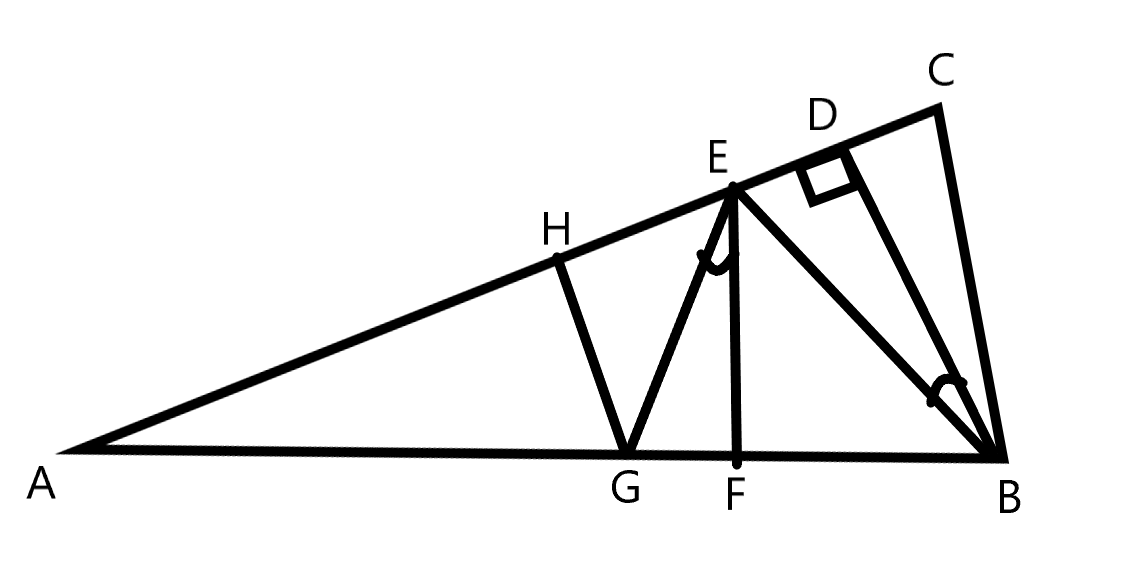
\includegraphics[scale = 0.3]{TriangleAnnotated.png}
	\caption{Amare the ant will travel across triangle $\triangle\rm ABC$ on a path from points B to E to G to H.}
	\label{fig:triangleAnnotated}
\end{figure}

We will add several points to triangle $\triangle\rm ABC$ to describe the path that Amare will take. 

Amare could take any straight line path to side AC, but going towards point C takes Amare farther from side AB. Traveling directly to side AC would minimize that portion of the trip, but Amare can shorten later sections by traveling to a point E that lies closer to A. Therefore, we define the segment perpendicular to AC and passing through B with the point D. Amare travels to the point E on AD, and we define angle $\angle{\rm DBE}=\theta$. 

Similar logic applies to suggest that Amare could travel directly to side AB from point E, but should aim for a point G closer to A. As in the previous step, we can define the point F on AB via the segment perpendicular to AB that intersects E, and we define angle $\angle{\rm FEG}=\phi$. 

Finally, Amare should travel to AC directly, and so we define the point H on AC via the segment perpendicular to AC that intersects G. 

With the previous construction, shown in Fig. $\ref{fig:triangleAnnotated}$, Amare will take a partwise straight-line path from points B to E to G to H. We need to analyze the situation to find the values of $\theta$ and $\phi$ that will minimize Amare's distance traveled. 

The distance traveled is given by $\overline{BE} + \overline{EG} +\overline{GH}$. We will develop expressions for each length in turn.

We begin by looking at the right triangle $\triangle {\rm ABD}$. Since $\angle{\rm CAB}=15^\circ$ and $\overline{AB}=1$, we have $\overline{BD}=\sin(15^\circ)$. We can look at the right triangle $\triangle{\rm BDE}$, 
\begin{align*}
\overline{BE} &= \frac{\overline{BD}}{\cos \theta} \\
&= \frac{\sin(15^\circ)}{\cos\theta}.
\end{align*}

We can then look at the right triangle $\triangle{\rm BFE}$. Since $\angle{\rm ABD}=75^\circ$, we have $\angle{\rm EBF}=75^\circ-\theta$. By the right angle, $\overline{EF}=\overline{BE} \sin(\angle{\rm EBF})$. Turning to the right triangle $\triangle{\rm FEG}$, we can determine $\overline{EG}$, 
\begin{align*}
\overline{EG} &= \frac{\overline{EF}}{\cos \phi} \\
&= \frac{\sin(75^\circ-\theta)}{\cos \phi}\frac{\sin15^\circ}{\cos\theta}.
\end{align*}

We note that $\angle{\rm AEF}=75^\circ$, implying $\angle{\rm HEG}=\angle{\rm AEG} = 75^\circ-\phi$. Looking at the right triangle $\triangle{\rm EHG}$, we can express $\overline{GH}$, 
\begin{align*}
\overline{GH}&= \overline{EG}\sin(\angle{\rm GEH}) \\
&= \sin(75^\circ-\phi) \frac{\sin(75^\circ-\theta)}{\cos \phi}\frac{ \sin 15^\circ}{\cos\theta}.
\end{align*}

Putting everything together, and noting $\sin(75^\circ-x)=\cos(15^\circ+x)$, we can write the total distance traveled by Amare as 
\begin{align*}
d(\theta, \phi) &= \frac{\cos(15^\circ+\phi)}{\cos \phi} \frac{\cos(15^\circ+\theta)}{\cos\theta} \sin 15^\circ + \frac{\sin(15^\circ)}{\cos \phi} \frac{\cos(15^\circ+\theta)}{\cos\theta} + \frac{\sin(15^\circ)}{\cos\theta}.
\end{align*}

We recall from their definition that the appropriate domain for $\theta$ and $\phi$ are $[0, 75^\circ]$. At the extremes, we have $d(75^\circ, \phi) = 1$ for any $\phi$, and $d(0,0) = \sin(15^\circ)(1+\cos(15^\circ)+\cos^2(15^\circ))$. 

Using some calculus, we could find the minimum of the distance function over the domain. \href{https://www.wolframalpha.com/input/?i=minimize+\%28cos\%28pi\%2F12\%2Bphi\%29\%2Fcos\%28phi\%29*cos\%28pi\%2F12\%2Btheta\%29\%2Fcos\%28theta\%29*sin\%28pi\%2F12\%29\%2Bsin\%28pi\%2F12\%29\%2Fcos\%28phi\%29*cos\%28pi\%2F12\%2Btheta\%29\%2Fcos\%28theta\%29\%2Bsin\%28pi\%2F12\%29\%2Fcos\%28theta\%29\%29}{WolframAlpha} gives a local minimum at $(\theta, \phi)=(\pi/6, \pi/12) = (30^\circ, 15^\circ)$ with minimum distance $1/\sqrt{2}$. 

This minimum happens to be the side length of an isosceles right triangle with hypotenuse 1. This value is not a coincidence, as there is a \href{https://laurentlessard.com/bookproofs/triangle-trek/}{geometric proof} involving such a triangle that simplifies the solution for this problem. 

\end{document}